\chapter{Программная реализация модуля}

\section{Выбор технического средства решения задачи}

\section{Руководство пользователя}

\subsection{Установка JMeter}

Для начала необходимо скачать с сайта производителя zip архив, содержащий все необходимы для установки файлы,
а затем распаковать его на диске. Место установки JMeter далее будем называть JMETER\_HOME.

\subsection{Установка модуля amf-translator}

Чтобы подключить к JMeter модуль amf-translator, достаточно добавить jar-файл приложения в каталог JMETER\_HOME/lib/ext.

\subsection{Запуск приложения}

Приложение запускается с помощью файла jmeter.bat или ApacheJMeter.jar, находящихся в каталоге JMETER\_HOME/bin.

\subsection{Настройка прокси-сервера}

После запуска в окне приложения с левой стороны нам доступно дерево элементов. Чтобы создать прокси сервер
с поддержкой протокола AMF, необходимо правой кнопкой мыши кликнуть по элементу WorkBench,
а затем добавить элемент AMF Proxy Server (WorkBench > Add > Non-Test Elements > AMF Proxy Server).

\begin{figure}[ht]
\center{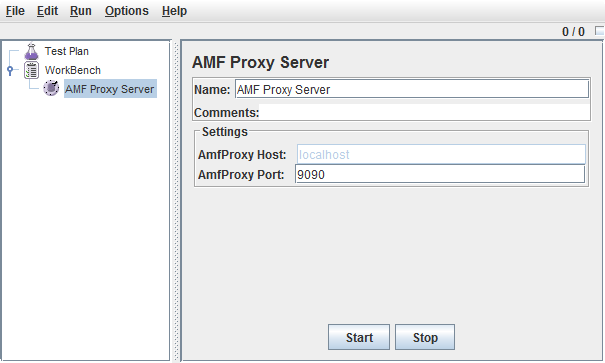
\includegraphics[height=120mm, width=160mm]{fig/development/proxySettings.png}}
\caption{Настройка прокси-сервера}
\label{ris:proxySettings.png}
\end{figure}

В поле AmfProxy Port необходимо указать номер порта, который будет слушать наш прокси сервер.
Если указать, например, 9090, то прокси-сервер будет запущен на localhost:9090.
Затем точно такие же настройки прокси-сервера устанавливаются в браузере, с помощью которого будет
производиться тестирование. Также стоит убедиться, что указанный Вами порт уже не занят другим приложением.

\subsection{Запись тестового сценария}

После того, как в AMF Proxy Server установлены все необходимые параметры, нажимается кнопка Start,
запускающая прокси-сервер.

\begin{figure}[h]
\center{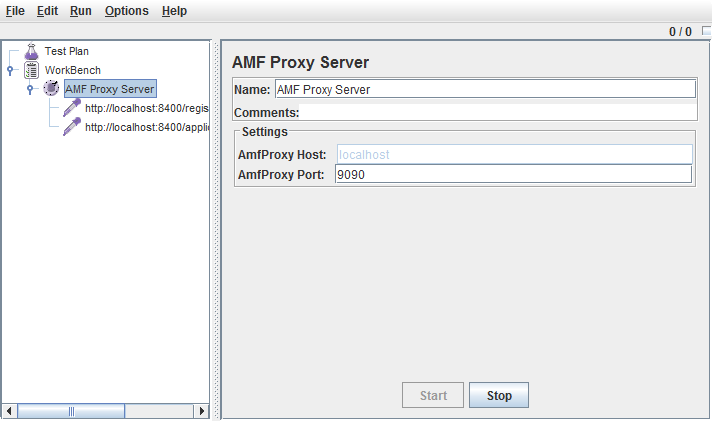
\includegraphics[height=120mm, width=160mm]{fig/development/proxyStart.png}}
\caption{Запуск прокси-сервера}
\label{ris:proxyStart.png}
\end{figure}

Затем тестируемое приложение открывается в браузере, для которого также
применены соответсвующие настройки прокси-сервера, и пользователь может выполнять с Flex приложением
необходимые операции, которые будут записываться AMF Proxy Server в виде элементов AMF RPC Sampler и в
дальнейшем могут быть перенесены в тест-план. Чтобы завершить запись тестовых запросов, необходимо
нажать кнопку Stop. После завершения записи тестов, все перехваченные запросы отображаются в дереве
элементов JMeter в качестве дочерних элементов AMF Proxy Server.

\subsection{Создание тест-плана}

Создание тест-плана в JMeter осуществляется следующим образом.
В первую очередь добавляется группа потоков - Thread Group (Test Plan > Threads (Users) > Thread Group).

\begin{figure}[ht]
\center{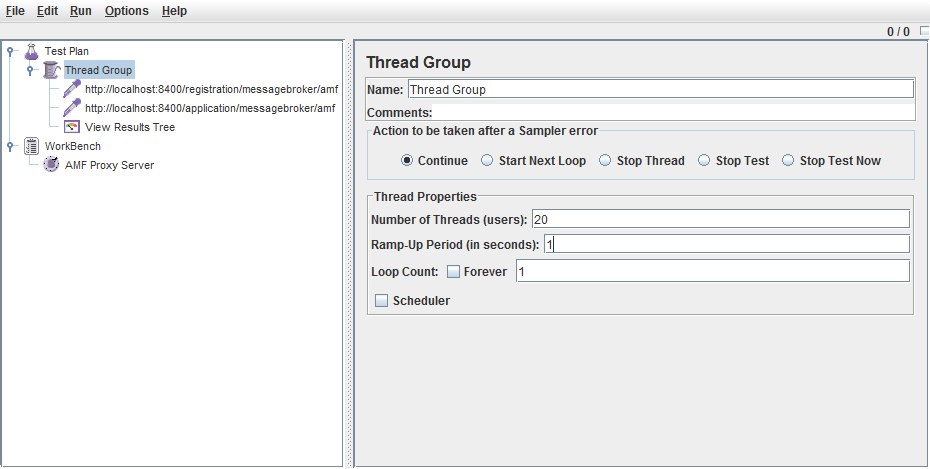
\includegraphics[height=120mm, width=160mm]{fig/development/testplan.png}}
\caption{Создание тест-плана}
\label{ris:testplan.png}
\end{figure}

Этот элемент является ключевым в тест-плане JMeter, именно его функционал отвечает за реализацию
нагрузочного тестирования --- многопоточного запуска последовательности тестовых шагов.
В данном элементе задается следующее:

\begin{enumerate}
\item Действия, которые будут производиться в случае, если в тест выполняется с ошибкой
(Action to be taken after a Sampler error);
\item Число потоков, в которое будут запускаться шаги тест-плана (Number of Threads);
\item Интервал, в течение которого будет запущено указанное в предыдущем параметре
число потоков (Ramp-Up Period);
\item Число повторений набора тестов (Loop Count);
\item Расписание запуска тестов (Scheduler).
\end{enumerate}

Затем в Thread Group в качестве дочерних элементов добавляются шаги тестов, которые
будут запускаться с указанными характеристиками. В нашем случае мы переносим элементы
AMF RPC Sampler, записанные с помощью прокси.

AMF RPC Sampler представляет собой форму для вызова процедур java-объектов на стороне
сервера. Чтобы вызвать метод удалённого объекта, необходимо заполнить следующие
поля: 

\begin{enumerate}
\item Endpoint Url - URL, по которому отправляется запрос
\item AMF Call - имя удалённого объекта и процедуы, которая должна быть вызвана; 
Например, если мы хоти вызвать у объекта registrationDestionation метод registerUser, 
в этом поле следует написать registrationDestination.registerUser;
\item Request Parameters - параметры метода, вызываемого у объекта (если они 
существуют).
\end{enumerate}

На Рис.~\ref{ris:amfSampler.png} представлен интерфейс AMF RPC Sampler.
\begin{figure}[ht]
\center{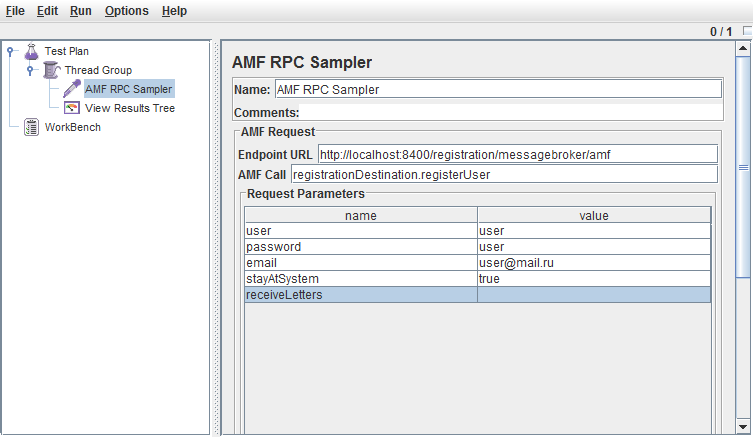
\includegraphics[height=120mm, width=160mm]{fig/development/amfSampler.png}}
\caption{Интерфейс элемента AMF RPC Sampler}
\label{ris:amfSampler.png}
\end{figure}
 
Помимо сэмплера в тест-план также следует добавить визуалайзер результатов, чтобы иметь возможность
отслеживать ход тестового сценария (Thread Group > Add > Listener ).
JMeter предлагает большой выбор таких элементов, для примера будем использовать View Results Tree.
После того как план сформирован, он может быть сохранён. (File > Save Test Plan As...)

\subsection{Запуск тестов}

Чтобы запустить содержимое элемента Test Plan, необходимо выбрать в основном меню Run > Start.
После заврешения прогона тестов результаты их выполнения можно наблюдать в View Results Tree.

\begin{figure}[ht]
\center{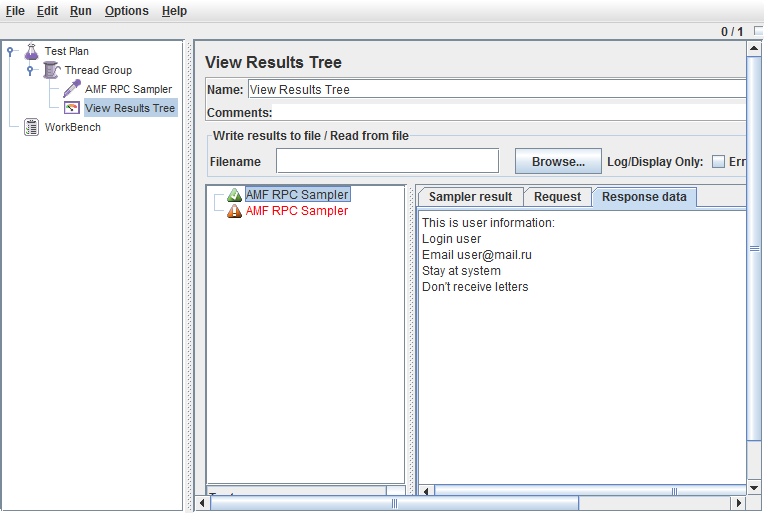
\includegraphics[height=110mm, width=160mm]{fig/development/testResults.png}}
\caption{Отображение результатов тестов в визуалайзере View Results Tree}
\label{ris:testResults.png}
\end{figure}

В правой части визуалайзера отображается дерево элементов тест плана и статус 
их выполнения - если элемент подсвечен зелёным цветом, то шаг выполнен 
успешно. В случае с AMF RPC Sampler это значит, что соединение с сервером было установлено 
и вызов метода удалённого объекта прошёл без ошибок. Иначе тест не считантся пройденным и 
элемент подсвечивается красным цветом. Также на вкладках слева предоставляется 
возможность просмотра отправленного запроса и полученного от сервера ответа.  

\section{Методика тестирования}